\documentclass[10pt,twocolumn,letterpaper]{article}

\makeatletter
\setlength{\@fptop}{0pt}
\makeatother

\usepackage{cvpr}
\usepackage{times}
\usepackage{epsfig}
\usepackage{graphicx}
\usepackage{amsmath}
\usepackage{amssymb}
\usepackage{csvsimple}
\usepackage{float}
\usepackage{subcaption}
\usepackage{tabularx}
\usepackage{multirow}
\usepackage{booktabs}
\usepackage[tableposition=top]{caption}

\usepackage[
sorting=none, 
block=ragged,
citestyle=ieee
]{biblatex}

\addbibresource{egbib.bib}
\renewcommand*{\bibfont}{\footnotesize}
\usepackage[breaklinks=true,bookmarks=false]{hyperref}

\cvprfinalcopy 

\def\httilde{\mbox{\tt\raisebox{-.5ex}{\symbol{126}}}}

\setcounter{page}{1}
\begin{document}

%%%%%%%%% TITLE
\title{Applied Machine Learning
Systems Report}

\author{Student Number: 15031625}

\maketitle
%\thispagestyle{empty}

%%%%%%%%% ABSTRACT
\begin{abstract}
   Most modern approaches for image recognition use some form of a convolutional neural network (CNN) to obtain state of the art results. In this paper, the power of CNNs is leveraged to perform unsupervised noisy image filtering and several supervised classification tasks on an image dataset of faces. The initial dataset contains noisy, non-facial images which must be filtered prior to classification. For filtering, a pre-trained CNN from literature (ResNet50 \cite{DBLP:journals/corr/HeZRS15}) is used to extract high-level features from each image. These features are then preprocessed and clustered, then the cluster containing the noisy images is removed. Following, two approaches are used to perform classification with CNNs, training a custom CNN from scratch, and using a pre-trained CNN to extract image features again to use for transfer learning to a linear classifer. Both methods obtain similar, high predictive accuracies for all classification tasks on an out-of-sample test set.
\end{abstract}

%%%%%%%%% BODY TEXT

\section{Introduction} \label{introduction}

The aim of this assignment is to perform several classification tasks on a dataset of 5000 images. The dataset mostly consists of images of both celebrity and cartoon faces. It also contains some mislabelled noisy images, primarily of nature scenes and blank backgrounds, which must be filtered out prior to training a model. Labels for each image are provided, consisting of integer values that represent whether the image contains someone smiling or not smiling, young or old, wearing glasses or not, a human or a cartoon, and the hair colour of the person. For example, a hair color label of '4' means the image is of a person with black hair and an eyeglasses label of '-1' means the person is not wearing glasses. The hair color for some of the images is set to -1, these are mislabelled and are later filtered from the dataset. A short snippet of the labels is shown as an example:
\resizebox{8cm}{!}{
\csvautotabular[respect all]{attribute_list_short.csv}
}
\vspace{5px}\\

Each label column represents a different classification task. These tasks are either binary classification, as in the case of the human, smiling, eyeglasses, and young columns, or multi-class classification for the hair color column. After filtering the noisy images out of the dataset, we want to train an appropriate machine learning model to accurately predict the label values of images in an out-of-sample test set.

All of the images are of the same file type (PNG) and are the same size (256 pixels by 256 pixels), which minimizes the amount of preprocessing that is necessary. However, the images have different color spaces, most being the 3-channel RGB, some the 4-channel RGBA, and a few are the 2-channel grayscale. The RGB color model represents the amount of red, green, and blue in each pixel. RGBA adds on a fourth dimension called the 'alpha' channel which represents the opacity of a pixel. As part of the preprocessing process, it is useful to convert all the images to a standard color space. For this task I want to preserve the color in the images, but keep dimensionality as small as possible. The opacity of the RGBA images is not necessarily useful for this task, therefore I will be using RGB for all the images. Additionally, RGB is the best colorspace to use with CNNs \cite{DBLP:journals/corr/MishkinSM16}. Once each image is loaded with the RGB color space, it will have the shape $(256, 256, 3)$. Considering our full dataset is quite large, it is useful to reduce the size of the image to speed up training \cite[p.34]{nixon2012feature}. This is accomplished by downsampling the image to a size of $(128, 128, 3)$, reducing the total size of the image by a factor of 4 while preserving most of the information present in the original. An image size of 128 by 128 was shown to be effective in \cite{DBLP:journals/corr/MishkinSM16}, further motivating the decision. Figure \ref{fig:downsample} demonstrates the minimal reduction in quality from downsampling. Finally, the RGB pixel values are normalized by scaling the pixel intensity to a range between 0 and 1, rather than between 0 and 255 which would be too high to train the model on \cite{cholletbuildingpowerful}, by dividing each value by $\frac{1}{255}$.

\begin{figure}[!htbp]
\begin{center}
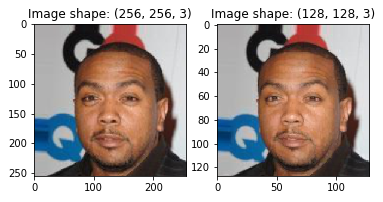
\includegraphics[width=1\linewidth]{downsample_comparison.png}
\end{center}
   \caption{Comparison of an original and downsampled RGB image. The original image has a shape of (256, 256, 3)
   and the downsampled image has a shape of (128, 128, 3). This represents a reduction in size by a factor of 4.}
\label{fig:downsample}
\end{figure}


\section{Proposed Algorithms} \label{algorithms}
This problem is divided into two separate tasks, filtering noisy images from the dataset and then training machine learning models to perform classification on the remaining images. The following subsections describe and provide a brief background for my proposed approaches to each. Background for minor topics that are not the focus of the report, such as linear classifiers, is excluded for brevity. 

\subsection{Image Filtering} \label{filtering}
 As the noisy images are mislabelled, the filtering task must rely on some form of unsupervised learning to group the images and remove those that are different from the rest of the dataset. My proposed approach for this task is to extract the features from the images with a pre-trained image classification model, map those features to the 2-D plane, and then perform clustering on that mapping. The cluster of images containing the noisy images would then be removed from the dataset.

 Data representation is one of the biggest influences on clustering performance, and using just the RGB pixel values will likely result in poorly chosen clusters. Feature extraction is a dimensionality reduction process that involves obtaining a derived vector representation of the image, that takes up less resources than the raw RGB data. Extracting the features is useful because if the representation of the images is good, then even a simple clustering algorithm like K-means will be able to find compact and isolated clusters \cite{JAIN2010651}. One approach to feature extraction is to use a deep convolutional network (CNN) that has been pre-trained for classification on a large image dataset (e.g. ImageNet \cite{imagenet_cvpr09}) to obtain the activation values (features) of one of the hidden layers in the network \cite{sharif2014cnn}\cite{karpathy_2018_transfer}. The earlier the hidden layer appears in the network, the more generic the extracted features will be, therefore it is common to use the activations of the hidden layer directly before the final fully-connected layer (the linearly separable classifier), which are known as the 'CNN codes' \cite{karpathy_2018_transfer}. The results with pre-trained CNN feature extraction have been shown to be comparable with other state-of-the-art feature extraction methods \cite{sharif2014cnn}.
 
 Once the CNN codes have been obtained for each image, the next task is to embed these high-dimensional vectors in a 2-D space. The resulting embeddings can then be plotted on a grid and clustered on their distances from each other. t-Distributed Stochastic Neighbour Embedding (t-SNE) is a popular embedding technique that is particularly suited for this task, producing visually appealing results for high dimensionality datasets. \cite{maaten2008visualizing}\cite{karpathy_2018_visualizing}. The original authors of the t-SNE method first apply principal component analysis (PCA), another dimensionality reduction technique, to reduce the dimensionality of the data (down to 30) prior to input into t-SNE. This helps speeds up the t-SNE computation and suppress some noise that arises from the transformation \cite{maaten2008visualizing}.

Lastly, once the 2-D mapping of the CNN codes has been calculated, we can use the K-means algorithm to cluster the image representations by squared Euclidean distance. K-means was selected because it is the simplest method for clustering analysis, but still works well when the extracted features are good \cite{JAIN2010651}. It is an iterative algorithm which aims to group $n$ data samples into $k$ clusters. The first step in the algorithm is to choose $k$ data samples at random from the dataset to act as an initial set of centroids. Then for the second step, each data sample in the dataset is assigned to its closest centroid, creating the first iteration of clusters. For the third step, the centroid of each of these clusters is recomputed. These second and third steps are repeated until there are no more changes to the centroids \cite{rodrigues2018AMLS}\cite{JAIN2010651}. The ideal number of clusters can be found with the elbow method, which is a visual method that compares the number of clusters, $k$, with the sum of squared distances (the cost function). When a plateau or 'elbow' of the cost function is observed at a certain $k$, then that is the $k$ value that should be selected \cite{rodrigues2018AMLS}\cite{kodinariya2013review}. After clustering with K-means, the final step for the filtering task is to simply identify the cluster containing the noisy images and remove all images in that cl.

\subsection{Image Classification} \label{classification}

Once the noisy images are filtered, the supervised learning classification tasks can begin to be carried out. Both of my approaches for classification use the widely popular convolutional neural networks (CNNs or ConvNets). In this section, I give a concise background of CNNs, with topics such as output functions and optimization algorithms for training (e.g. Adam) not covered for brevity. More in depth and mathematical coverage of CNNs can be found in the cited literature.

CNNs are made up of a sequence of several stacked layers, much like traditional neural networks. However, traditional networks employ full connectivity in each of their layers, which is not appropriate for image processing as the number of parameters to train would be too high. CNNs on the other hand are designed specifically for processing data with a grid-like representation, such as RGB image data (3D grid) \cite[p.321]{goodfellow2016deep}.
CNNs are used in many of the top performing image classification techniques, achieving almost half the error rates of previous methods \cite{lecun2015deep}\cite{krizhevsky2012imagenet}. In fact, it has been demonstrated that CNNs provide a considerable improvement for facial recognition tasks similar to this assignment \cite{taigman2014deepface}. CNNs are particularly effective in image recognition/classification because they are based on a simplified model of the primary visual cortex, the area of the brain that performs advanced visual processing \cite[p.353]{goodfellow2016deep}.

As their name implies CNNs heavily employ the convolution operation, which is applied in the convolutional layers. The convolutional layer's learnable parameters are a set of filters. These filters are arrays of a small height and width (generally 3 pixels by 3 pixels), along with the same depth of the images (3 in the RGB case). We slide/convolve the filter along the width and height of an input image and compute the dot-product between the filter and the current section of the image (called the receptive field). A 'stride' parameter defines how many pixels we slide the filters by each time (generally 1 or 2). The dot-product values for each receptive field are processed by a non-linear activation function (e.g. ReLU, tanh) and put into a 2D 'feature map' array. The network can then learn to associate these feature maps with the image features that activate them. Since we have multiple filters in each convolutional layer, they will produce multiple feature maps, forming the layer's output. Further, by cascading multiple convolutional layers we can obtain feature maps of higher level image features for each layer \cite{karpathy_2018_cnn}\cite[Ch.6]{nielsen2015neural}\cite[Ch.9]{goodfellow2016deep}\cite{andreopoulos2018CNN}.

CNNs also contain pooling layers, which are used right after a convolutional layer. Pooling layers are used to reduce the number of parameters in a network. Essentially, they resize the feature map outputs of a convolutional layer spatially by sliding a filter (commonly 2x2) along the feature map and taking the maximum or average activation value in the filter. With a filter size of 2x2 and a stride of 2, this will get rid of 75\% of the activations in each feature map, reducing the number of parameters and network overfitting \cite{karpathy_2018_cnn}\cite[Ch.6]{nielsen2015neural}\cite[Ch.9]{goodfellow2016deep}\cite{andreopoulos2018CNN}.

After passing through several stacked convolutional and pooling layers, one or more fully connected layers (as used in traditional neural nets) are used to map the activations of the previous layers to the output neurons of the network. The activations are mapped to the same number of neurons as output classes (2 for binary classification), with each neuron representing one of the output classes. As the name implies, the neurons in a fully connected layer have full connections to the neurons in the preceding layer, meaning they can be responsible for much of the complexity present in a CNN. If necessary, to reduce the number of parameters, fully connected layers can be converted convolutional layers that perform the same function \cite{karpathy_2018_cnn}\cite[Ch.6]{nielsen2015neural}\cite[Ch.9]{goodfellow2016deep}\cite{andreopoulos2018CNN}.

Non-linear activation functions, as briefly mentioned before, are used throughout the CNN architecture to introduce non-linearity to the network parameters, allowing the network to select non-linear decision boundaries. The most common activation function used in modern networks is the rectified linear unit (ReLU). ReLU is defined by the function $g(z) = max(0,z)$, which removes any negative values from the feature map. The ReLU function is much more efficient than other common activation functions like sigmoid or tanh, speeding up training. \cite{karpathy_2018_cnn}\cite{karpathy_2018_nn1}\cite[Ch.6]{nielsen2015neural}\cite[Ch.6, Ch.9]{goodfellow2016deep}\cite{andreopoulos2018CNN}. 

Dropout layers can be added to a network as a simple regularization technique to help prevent overfitting. During training, dropout layers set a random portion of the neurons of the preceding layer to 0, essentially dropping them. The probability that a neuron will be dropped is controlled by the dropout rate parameter. For example, setting the dropout rate to 0.5 will result in each neuron having a 50\% chance of being dropped in each iteration. Applying dropout leads to a 'thinned' network with only the neurons that were not dropped. During testing, all activations are used without dropout, but their weights are reduced by the dropout rate  \cite{srivastava2014dropout}\cite{karpathy_2018_nn2}\cite[p.258]{goodfellow2016deep}\cite{andreopoulos2018CNN}.

My first proposed approach for classification is to design a custom CNN architecture with these layers and train the network from scratch. However, in reality most people choose not to train a CNN from scratch, rather a technique called transfer learning is preferred \cite{karpathy_2018_transfer}. Transfer learning is when a pre-trained CNN like ResNet50 \cite{DBLP:journals/corr/HeZRS15} is used to extract CNN codes (high-level features) which are used to train a linear classifier (e.g. linear SVM) \cite{karpathy_2018_transfer} to predict on custom image labels. This method produces state-of-the-art image classification results, with a substantially shorter training time \cite{sharif2014cnn}. Therefore, I also propose using transfer learning to obtain benchmark results with a large and high performing model from literature.

\section{Implementation} \label{implementation}
\subsection{Image Filtering}
\label{image_filter_implementation}

Several external Python libraries were used to develop the proposed filtering algorithm in section \ref{filtering}. Scikit-learn \cite{scikit-learn} was used for its PCA, T-sne and K-means functions. Keras \cite{chollet2015keras} was used for its CNN models pre-trained on ImageNet and image pre-processing functions. Further, Matplotlib \cite{Hunter:2007} was used to generate various plots. Finally, NumPy \cite{numpy} and Pandas \cite{mckinney-proc-scipy-2010} were used to accommodate data processing and manipulation.

Keras includes many models for image classification already trained on ImageNet \cite{imagenet_cvpr09}, a database of over 14 million labelled images. After a few initial tests, I settled on using a 50 layer residual network, ResNet50 \cite{DBLP:journals/corr/HeZRS15} to extract the image features. ResNet50 is not exceptionally large with 25,636,712 parameters (the largest net available has 143,667,240), but still has great predictive performance. It was chosen because residual networks are among the top performing models in image recognition due to their unique 'skip connections' \cite{DBLP:journals/corr/HeZRS15}
.

I then iterated through each image in the dataset and extracted their CNN codes with ResNet50 using max pooling, with its final dense layer removed. Max pooling is preferred over average pooling because it generally results in better performance \cite{karpathy_2018_cnn}. All the extracted feature vectors are stored then processed through a PCA and T-sne pipeline. PCA is used first to reduce the number of components in the feature vectors to 30 as suggested in \cite{maaten2008visualizing}. Then T-sne is used to map these reduced dimensionality features to the 2D plane.

Now that a 2-D interpretation of the CNN codes is obtained, K-means clustering can be performed. First we find the optimal number of clusters with the elbow method, by fitting K-means on the features for 1 to 15 clusters, and plotting the number of clusters against the the K-means cost function (sum of square distances). The elbow method plot is shown in figure \ref{fig:elbow}. Although there is no clear 'bend' in the plot, the decrease in the K-means cost function from adding more clusters becomes marginal at around $k=5$ ($k=6$ would be appropriate as well). The results of K-means with $k=5$ is shown in figure \ref{fig:clusters}. By checking the cluster of one of the noisy images, we find that cluster 4 should contain them all. The images in cluster 4 are then removed from the dataset. Finally, from manual inspection of the removed and remaining images, all 435 noisy images were successfully filtered out with no false positives.

\begin{figure}[!htbp]
\begin{center}
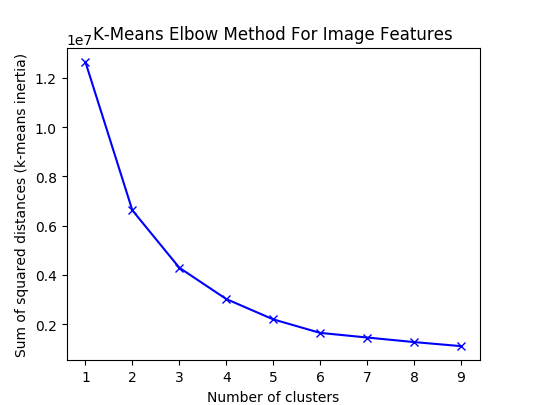
\includegraphics[width=1\linewidth]{elbow_method.png}
\end{center}
   \caption{K-means elbow method plot for the features extracted from the images. The number of clusters used for K-means is plotted against the sum of squared distances (called inertia in Scikit-learn)}
\label{fig:elbow}
\end{figure}

\begin{figure}[!htbp]
\begin{center}
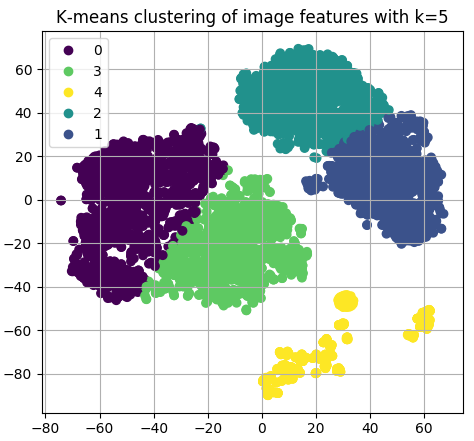
\includegraphics[width=0.9\linewidth]{clusters.png}
\end{center}
   \caption{K-means clustering with $k=5$ on the image features mapped to the 2D plane. Cluster 4 contains all the noisy images.}
\label{fig:clusters}
\end{figure}

\subsection{Image Classification}
\subsubsection{CNN classifier}
\label{CNN_Classifier_Implementation}
To implement the CNN classifier, I used the Keras \cite{chollet2015keras} library to create, train, and evaluate the CNN model and for its image preprocessing functions. Numpy \cite{numpy} and Pandas \cite{mckinney-proc-scipy-2010} were used for data manipulation and storage. Scikit-learn \cite{scikit-learn} was used to obtain various metrics of the CNN predictions. Lastly, Matplotlib \cite{Hunter:2007} was used to generate several plots.

The filtered image dataset was split into training, validation, and test sets with a randomized 60/20/20\% split as recommended in \cite{splittingsetsng} for datasets with less than 10,000 samples. This means that the training set will contain a random 60\% of the images, the validation set 20\%, and the test set contains the remaining 20\%. This split assigns many images for training (2739 images), while still leaving aside enough images for validation and testing (both 913 images) to sufficiently capture the variance present in the whole dataset and accurately evaluate the model.

The final CNN network architecture is shown in figure \ref{fig:architecture} in section \ref{additional_figures}. As shown, the layout of the network consists of several 2D convolutional layers with ReLU activation, 2D Max Pooling layers and dropout layers stacked together. These are followed by a flatten layer, a fully-connected dense layer with ReLU activation, and a final dense layer to map weights to classes. If the task is binary classification, the final dense layer has a sigmoid output function with binary crossentropy loss \cite[p.182]{goodfellow2016deep}. For a multi-class classification task, the final dense layer has a softmax output with categorical crossentropy loss \cite[p.184]{goodfellow2016deep}. The network has 6,507,617 parameters in total. 

The design used is based on the example given in \cite{gupta_2017} and is essentially a smaller version of AlexNet \cite{krizhevsky2012imagenet}. This repeating stack of layers is among the most common architectures for CNNs \cite{karpathy_2018_cnn}. The ReLU activation function is used for the convolutional layers because it is the default recommendation for modern networks \cite[p.174]{goodfellow2016deep}. The convolutional layers were set to have 32 or 64 small 3x3 filters with a stride of 1x1. Some have padding that keeps the output shape identical to the input shape as recommended in \cite{karpathy_2018_cnn}. The max pooling layers have a pool size of 2x2 and a stride of 2x2, again per \cite{karpathy_2018_cnn}. Multiple fully connected layers were used near the output, as was done in the AlexNet architecture \cite{krizhevsky2012imagenet}. The first fully connected dense layer's function is to act as a high level feature extractor. It uses ReLU activation and has 512 neurons, chosen not to be particularly high (AlexNet uses 2048 neurons in each fully connected layer \cite{krizhevsky2012imagenet}) as fully connected layers are responsible for most of the parameters present in the network. Finally, the second fully connected dense layer maps the image features to the predicted class of the image. For multiclass classification, this layer has the same number of neurons as there are classes. Otherwise for binary classification, it contains only a single neuron.

I settled on this design by initially testing several similar, but shallower architectures which underfit on some of the more difficult classification tasks. I managed to prevent underfitting by increasing the model's capacity \cite[p.111]{goodfellow2016deep} by adding more 2D convolutional layers and increasing the number of filters in the last two convolutional layers from 32 to 64. I avoided making the network too large in order to keep the training time from being exceedingly long \cite{karpathy_2018_nn1}. However, having a deeper network initially resulted in some overfitting, leading to poor model generalization and affecting validation and testing accuracy. To alleviate this I added dropout regularization with a rate of 0.25 to several lower layers as done in \cite{gupta_2017}, in addition to an existing dropout layer at the output with a recommended default (and close to ideal) dropout rate of 0.5 \cite{srivastava2014dropout}. Using dropout in lower layers is useful because it provides a noisy input for the later fully-connected dense layer, preventing overfitting \cite{srivastava2014dropout}.

The network was trained for each task with the Adam optimizer \cite{DBLP:journals/corr/KingmaB14}, as recommended in \cite{karpathy_2018_nn3}. The images' raw RGB pixel values were fed to the network with Keras's flow from directory generator, with the images downsampled to a shape of $(128, 128, 3)$ to speed up training. Further, each pixel value was scaled to a range between 0 and 1, because the CNN will have trouble learning with the default range of 0 and 255. No further image preprocessing was done, as customary for CNNs \cite{DBLP:journals/corr/MishkinSM16}. The model is trained with randomized batches of 32 images, which is the recommended default batch size value in \cite{DBLP:journals/corr/abs-1206-5533}. Batch size primarily affects model training time and not model performance \cite{DBLP:journals/corr/abs-1206-5533}, therefore it is not a critical hyperparameter to tune. Other Adam hyperparameters are set to the authors' recommended values (learning rate=0.001, $\beta_1$=0.9, $\beta_2$=0.999, $\epsilon$=1e-08) \cite{DBLP:journals/corr/KingmaB14} automatically in Keras. Although Adam is an adaptive learning rate method, I further use learning rate scheduling \cite{karpathy_2018_nn3} to automatically reduce the Adam learning rate once the validation loss does not improve by at least 0.01 in an epoch during training. Further, I use one of the most common forms of regularization and hyper parameter tuning, early stopping \cite{SrihariEarlyStopping}\cite{HintonBengioYannDeepLearningSlides}, to stop training early if the validation loss does not improve by at least 0.001 in an epoch. After early stopping, the model weights from the epoch with the lowest validation loss are restored instead of the last training iteration \cite{SrihariEarlyStopping}.

A large difference between the training and validation loss is an indicator for whether the model was overfit for a particular task \cite{karpathy_2018_nn3}. Additionally, If the validation loss is lower for a later epoch than an earlier one, that means the trained weights were restored to that earlier epoch. For each of these classification tasks, the final validation accuracy (after restoring weights to the best epoch) is close to the training accuracy, indicating that there was little overfitting of the network. Further, as the final training and validation accuracy for each task is high (after restoring weights to the best epoch), it shows the network was likely not underfit either \cite[p.115]{goodfellow2016deep}\cite{andreopoulos2018CNN}. The full training and validation loss/accuracy curves for each classification task can be seen in figure \ref{fig:learning_curves} in section \ref{additional_figures}. 

\subsubsection{Transfer learning classifier}

To implement the transfer learning classifier, I used the Keras \cite{chollet2015keras} library for its CNN models pretrained on ImageNet. Additionally, Numpy \cite{numpy} and Pandas \cite{mckinney-proc-scipy-2010} were used for data manipulation and storage. Lastly, Scikit-learn \cite{scikit-learn} was used to implement and train the linear SVM classifer on extracted image features and to obtain various performance metrics. 

As I had prior success with ResNet50 in section \ref{image_filter_implementation}, I used it again to extract the CNN codes of all the images. Each CNN code is a 2048 length vector of floats. CNN codes were extracted rather than lower-level features from earlier layers because our dataset is similar to the 'person' images in ImageNet \cite{imagenet_cvpr09}, meaning higher-level features will still be relevant \cite{karpathy_2018_transfer}. ResNet50 was left as-is without fine-tuning the weights. Fine-tuning is not recommended when the dataset is small in order to avoid overfitting \cite{karpathy_2018_transfer}.

The extracted CNN codes, along with the corresponding image labels for each task, were used to train and evaluate a linear SVM classifier. The same test set used in section \ref{CNN_Classifier_Implementation} was also used here to remove any influence of which images were in the test set on the results. The SVM class weights were balanced based on each classes frequency. Hyperparameter tuning in the form of randomized search was performed on the SVM's $C$ parameter, with the values of $C$ randomly sampled from a continuous scaled exponential function over 10 iterations. Randomized search was used because it is more efficient than grid search \cite{karpathy_2018_nn3}. 3-fold cross-validation was used for the randomized search, rather than using an explicit validation set as in section \ref{CNN_Classifier_Implementation}, because it is much simpler to implement with the Scikit-learn library. Finally, once the best value of $C$ is found with cross-validation, the model is refit on the test set to obtain the final predictive results.

\section{Experimental Results} \label{results}
\begin{table}[!htbp]
    \caption{Testing accuracy results of the custom CNN architecture and transfer learning with ResNet50 pretrained on ImageNet. Both were evaluated on the same out-of-sample test set.}
    \begin{tabularx}{\columnwidth}{X|X|X}
        \hline
        Task          & Custom CNN & ResNet50\\
        \hline
        1) Smiling    & 0.9288     & 0.9124\\
        2) Young      & 0.8883     & 0.8697   \\
        3) Eyeglasses & 0.9989     & 0.9824\\   
        4) Human      & 1.0000     & 1.0000\\
        \hline
        5) Hair Color & 0.8912     & 0.9385 \\
    \end{tabularx}
    \label{table: simulation parameters}
\end{table}

The testing accuracy of both the custom CNN model and the ResNet50 transfer learning model for all classification tasks are shown in table \ref{table: simulation parameters}. An identical test set was used to evaluate both models, which obtained similar results. The custom CNN performed slightly better for the 'smiling', 'young', and 'eyeglasses' tasks. Both models achieved 100\% accuracy for the simple 'human' task. However, ResNet50 transfer learning performed better on the 'hair color' task by more than 4\%. The confusion matrices for this task, shown in tables \ref{fig:hair_matrix} and \ref{fig:hair_transfer_matrix} in section \ref{additional_figures}, indicate that the custom CNN model particularly struggled with a hair color label of 0 (bald), whereas the ResNet50 model did not. Further, both models struggled on the difficult 'young' task, with the custom CNN obtaining 88.83\% accuracy and the transfer learning classifier model obtaining 86.97\% accuracy. 

Transfer learning with trained image classifiers from literature generally achieves state of the art results \cite{sharif2014cnn}, therefore it is expected that the ResNet50 transfer learning model performance would be close to the highest possible for a given classification task. As the custom CNN model obtained very similar results, we can conclude that it was largely successful in learning the classification tasks. However, the custom CNN's lower performance on the hair color task may indicate that it was somewhat underfit. This underfitting can be reduced by adding more layers to the model until the test accuracy stops improving \cite{DBLP:journals/corr/abs-1206-5533}. However, adding too many layers may cause optimization of the network to be difficult, leading to degradation in training error \cite{DBLP:journals/corr/HeZRS15}. In that case, 'skip connections' such as those found in residual networks \cite{DBLP:journals/corr/HeZRS15} can be used to stack even more layers without making training too difficult. Further, when both models obtain an imperfect accuracy on the same task, it may be due to the task being particularly difficult. For example, classifying whether someone is young looking is largely subjective and the features that make a person 'young' may be not be fully apparent to the models. Additional accuracy bottlenecks for both models arise from the mislabelling of some of the images in the dataset, where for example someone who is labelled as being old is actually young.

\section{Conclusion} \label{conclusion}

The custom CNN model defined in section \ref{CNN_Classifier_Implementation} produced comparable results to the ResNet50 transfer learning model. As transfer learning with pre-trained models from literature produces state of the art results \cite{sharif2014cnn}, we can conclude that the custom CNN learned the classification tasks successfully. Despite the success of the custom CNN here, in practice few people train a CNN from scratch \cite{karpathy_2018_transfer}. This is justified here because both models obtained similar accuracy for each task, but the transfer learning method took much less time to develop, tune, and train. Therefore, for similar tasks in the future I would recommend transfer learning.

If training a CNN from scratch is preferred, I would make some adjustments to the methods used. As the custom CNN scored an accuracy of 4\% less than the transfer learning model for the hair color task, we can assume the custom CNN was underfit. I would reduce this underfitting by adding more layers to the CNN architecture until there is no more improvement in test accuracy \cite{DBLP:journals/corr/abs-1206-5533}.  Additional improvements can be made by using augmented images (e.g. flipped, sheared, rotated, etc.) for training, which is a regularization technique that increases the train set size and reduces overfitting \cite{DBLP:journals/corr/abs-1712-04621}. Lastly, I would reduce the complexity of the custom CNN architecture by converting any fully-connected layers into convolutional layers, reducing the number of parameters and decreasing training time \cite{karpathy_2018_cnn}.

\section{Related Work}\label{related_work}

Most of the modern methods for image classification and object recognition use convolutional neural networks, as done in this paper. However, the CNN architecture used for this assignment is generally much simpler than those found in literature. One similar but deeper and wider architecture, AlexNet \cite{krizhevsky2012imagenet}, was published in 2012. The AlexNet architecture is made up of five convolutions layers (some followed by max-pooling layers), and three fully-connected layers of which dropout regularization follows the first two. AlexNet greatly outperformed all other models at the time on the ImageNet database. The authors note that the network depth was very important to obtaining these top results, with the predictive accuracy dropping by 2\% if any of the middle convolutional layers are removed. Further, the authors found that CNNs train several times faster when using ReLU activations rather than saturating functions like tanh. The promising results with AlexNet paved the way for an explosion of interest in deep learning for image recognition tasks. 

A newer, novel architecture for image recognition called residual networks was published in 2015 \cite{DBLP:journals/corr/HeZRS15}. Prior results such as AlexNet had focused on stacking many layers together to improve accuracy. However, the authors of residual networks found issue with this technique, showing that regular CNNs have higher training error as their depth increases because they become increasingly harder to optimize. Residual networks solve this problem by using 'shortcut connections' to skip layers and avoid non-linear activation functions, thus avoiding any vanishing gradients and allowing low-level features to flow deep into the network. The results with residual networks were state-of-the-art and beat out all other models on ImageNet at the time. Additionally, I personally had excellent results using a pretrained 50 layer residual network (ResNet50) to extract image features throughout this assignment.

A review of several improvements on CNN architectures for image recognition was published in 2016 \cite{DBLP:journals/corr/MishkinSM16}. This paper evaluates several choices that can be made in CNN architectures including the activation function, pooling type, and network layers. It does not cover any of the advancements shown with residual networks. Their results were obtained by testing adjustments on several networks from literature (CaffeNet128, CaffeNet224, VGGNet128 and GoogleNet128). Important recommendations based on the results include using ReLU (or ELU if batch normalization is used) as the activation function, reading images with an RGB color space, using linear learning rate decay during training, and using a sum of average and max pooling. Additionally, they recommend using a batch-size of 128 or 256 and converting fully-connected layers to convolutional layers. In the future, some of these suggestions can be used to improve the results of my CNN model.
\newpage
\section{Code Base}

The code base for this report be found at: \\
Google Drive: https://goo.gl/wXERtg\\
GitHub: https://github.com/IlyasI/AMLSassignment.

\section{Additional Figures and Tables}
\label{additional_figures}

\begin{figure}[!htbp]
\begin{center}
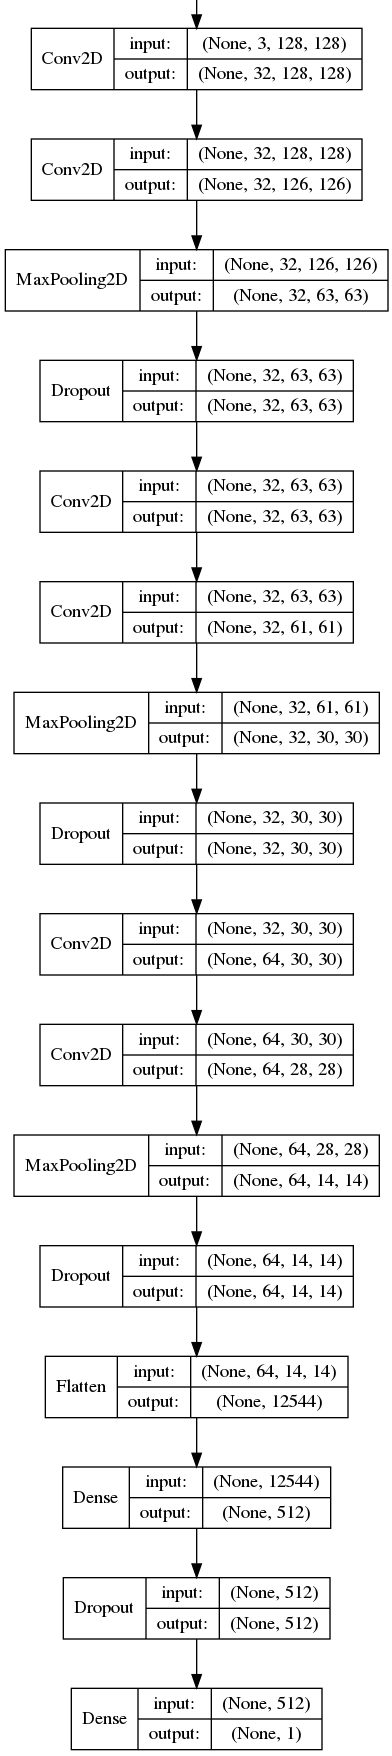
\includegraphics[height=17cm]{model.png}
\end{center}
   \caption{Final CNN classifier architecture with the input and output shapes shown for each layer. The ReLU and Sigmoid/Softmax functions are excluded for brevity.}
\label{fig:architecture}
\end{figure}

\begin{figure*}[!htbp]
  \centering
  \vspace*{-2cm}
  \begin{subfigure}[t]{.45\linewidth}
    \centering
    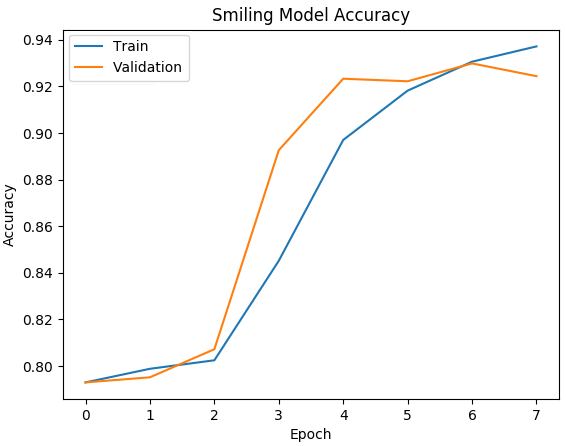
\includegraphics[width=\linewidth, height=4.8cm]{Smiling_model_accuracy.png}
    %\caption{Training and validation accuracy plotted per epoch for the 'smiling' task.}
  \end{subfigure}
  \hfill
  \begin{subfigure}[t]{.45\linewidth}
    \centering
    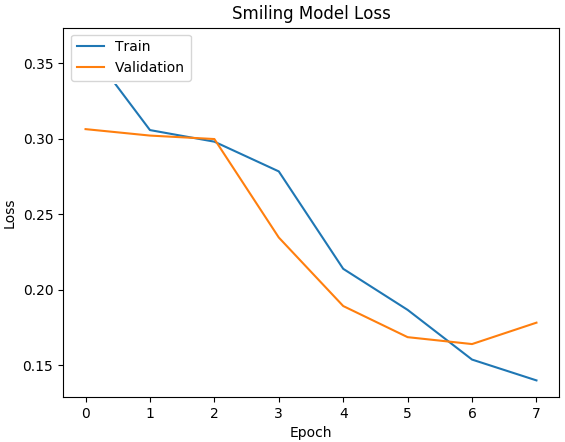
\includegraphics[width=\linewidth, height=4.8cm]{Smiling_model_loss.png}
    %\caption{Training and validation binary crossentropy loss plotted per epoch for the 'smiling' task.}
  \end{subfigure}

  \begin{subfigure}[t]{.45\linewidth}
    \centering
    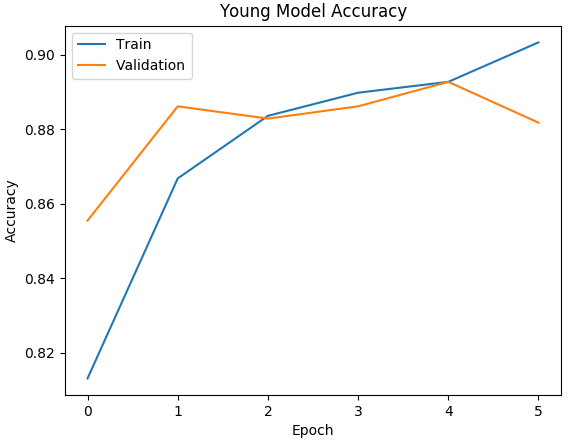
\includegraphics[width=\linewidth, height=4.8cm]{Young_model_accuracy.png}
    %\caption{Training and validation accuracy plotted per epoch for the 'young' task.}
  \end{subfigure}
  \hfill
  \begin{subfigure}[t]{.45\linewidth}
    \centering
    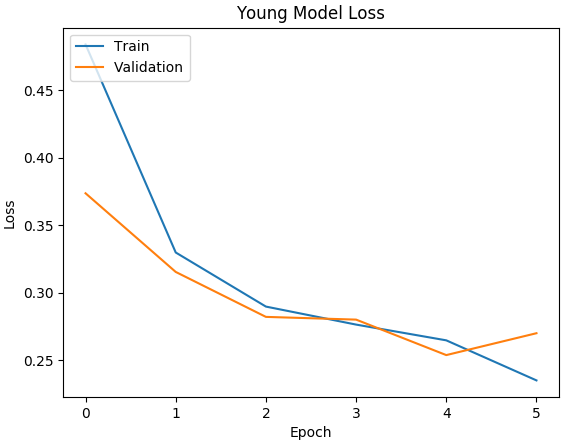
\includegraphics[width=\linewidth, height=4.8cm]{Young_model_loss.png}
    %\caption{Training and validation binary crossentropy loss plotted per epoch for the 'young' task.}
  \end{subfigure}

  \begin{subfigure}[t]{.45\linewidth}
    \centering
    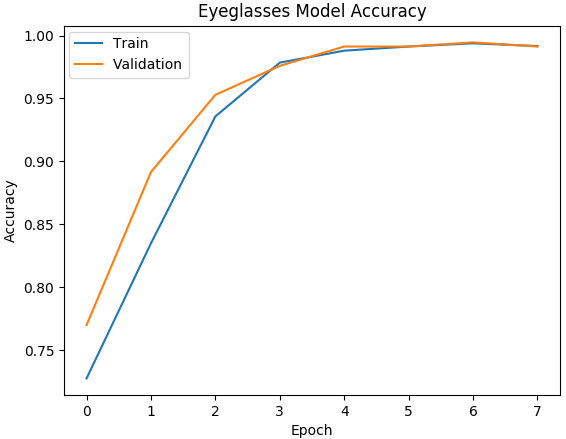
\includegraphics[width=\linewidth, height=4.8cm]{Eyeglasses_model_accuracy.png}
    %\caption{Training and validation accuracy plotted per epoch for the 'eyeglasses' task.}
  \end{subfigure}
  \hfill
  \begin{subfigure}[t]{.45\linewidth}
    \centering
    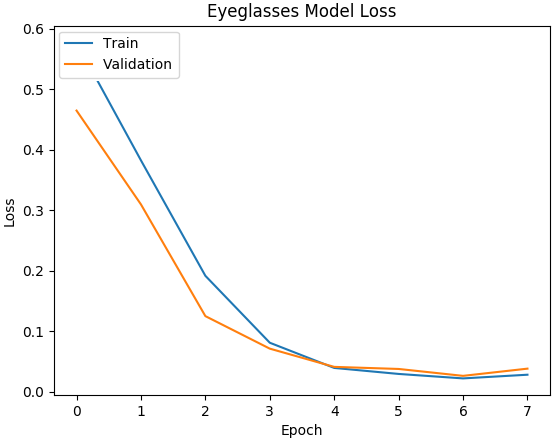
\includegraphics[width=\linewidth, height=4.8cm]{Eyeglasses_model_loss.png}
    %\caption{Training and validation binary crossentropy loss plotted per epoch for the 'eyeglasses' task.}
  \end{subfigure}

  \begin{subfigure}[t]{.45\linewidth}
    \centering
    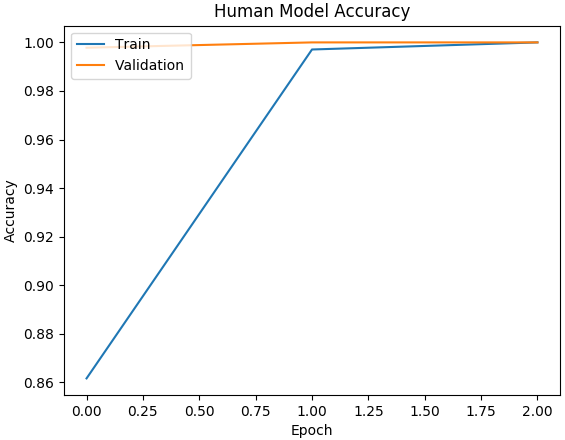
\includegraphics[width=\linewidth, height=4.8cm]{Human_model_accuracy.png}
    %\caption{Training and validation accuracy plotted per epoch for the 'human' task.}
  \end{subfigure}
  \hfill
  \begin{subfigure}[t]{.45\linewidth}
    \centering
    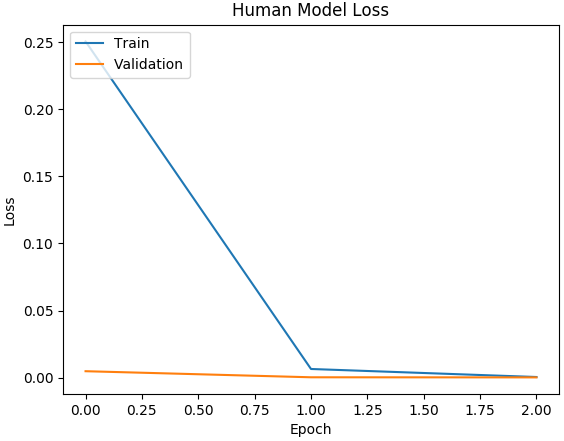
\includegraphics[width=\linewidth, height=4.8cm]{Human_model_loss.png}
    %\caption{Training and validation loss plotted per epoch for the 'human' task.}
  \end{subfigure}
  
    \begin{subfigure}[t]{.45\linewidth}
    \centering
    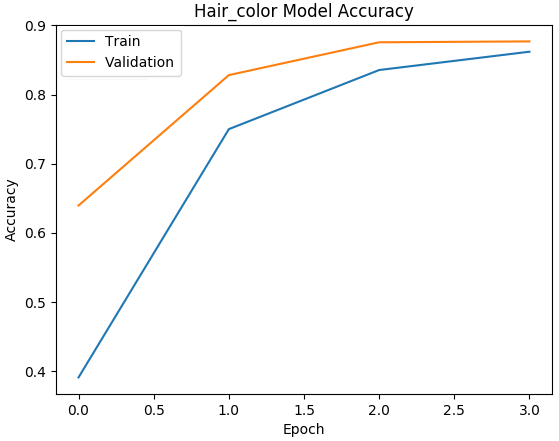
\includegraphics[width=\linewidth, height=4.8cm]{Hair_color_model_accuracy.png}
    %\caption{Training and validation accuracy plotted per epoch for the 'hair color' task.}
  \end{subfigure}
  \hfill
  \begin{subfigure}[t]{.45\linewidth}
    \centering
    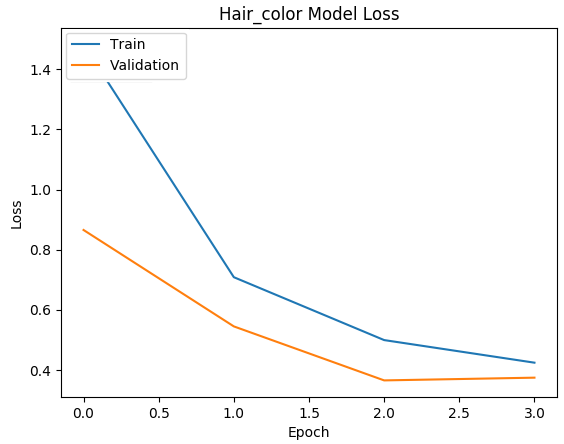
\includegraphics[width=\linewidth, height=4.8cm]{Hair_color_model_loss.png}
    %\caption{Training and validation categorical crossentropy loss plotted per epoch for the 'hair color' task.}
  \end{subfigure}
\caption{Training (blue) and validation (orange) accuracy and loss plotted against the training epoch for each of the classification tasks.}

\label{fig:learning_curves}

\end{figure*}

\begin{table}[p]
\begin{minipage}{.45\linewidth}
\centering
\caption{'Smiling' CNN classifier confusion matrix}
\label{fig:smiling_matrix}
\begin{tabular}{@{}cc|cc@{}}
\multicolumn{1}{c}{} &\multicolumn{1}{c}{} &\multicolumn{2}{c}{Predicted} \\ 
\multicolumn{1}{c}{} & 
\multicolumn{1}{c|}{} & 
\multicolumn{1}{c}{-1} & 
\multicolumn{1}{c}{1} \\ \hline
\multirow[c]{2}{*}{\rotatebox[origin=tr]{90}{Actual}}
& -1  & 155 & 36   \\[1.5ex]
& 1  & 29   & 693 \\ \hline
\end{tabular}
\end{minipage}\hfill
\begin{minipage}{.45\linewidth}
\centering
\caption{'Young' CNN classifier confusion matrix}
\label{fig:young_matrix}
\begin{tabular}{@{}cc|cc@{}}
\multicolumn{1}{c}{} &\multicolumn{1}{c}{} &\multicolumn{2}{c}{Predicted} \\ 
\multicolumn{1}{c}{} & 
\multicolumn{1}{c|}{} & 
\multicolumn{1}{c}{-1} & 
\multicolumn{1}{c}{1} \\ \hline
\multirow[c]{2}{*}{\rotatebox[origin=tr]{90}{Actual}}
& -1  & 102 & 90   \\[1.5ex]
& 1  & 12   & 709 \\ \hline
\end{tabular}
\end{minipage}
\end{table}

\begin{table}[!htbp]
\begin{minipage}{.45\linewidth}
\centering
\caption{'Eyeglasses' CNN classifier confusion matrix}
\label{fig:glasses_matrix}
\begin{tabular}{@{}cc|cc@{}}
\multicolumn{1}{c}{} &\multicolumn{1}{c}{} &\multicolumn{2}{c}{Predicted} \\ 
\multicolumn{1}{c}{} & 
\multicolumn{1}{c|}{} & 
\multicolumn{1}{c}{-1} & 
\multicolumn{1}{c}{1} \\ \hline
\multirow[c]{2}{*}{\rotatebox[origin=tr]{90}{Actual}}
& -1  & 644 & 0   \\[1.5ex]
& 1  & 1   & 268 \\ \hline
\end{tabular}
\end{minipage}\hfill
\begin{minipage}{.45\linewidth}
\centering
\caption{'Human' CNN classifier confusion matrix}
\label{fig:human_matrix}
\begin{tabular}{@{}cc|cc@{}}
\multicolumn{1}{c}{} &\multicolumn{1}{c}{} &\multicolumn{2}{c}{Predicted} \\ 
\multicolumn{1}{c}{} & 
\multicolumn{1}{c|}{} & 
\multicolumn{1}{c}{-1} & 
\multicolumn{1}{c}{1} \\ \hline
\multirow[c]{2}{*}{\rotatebox[origin=tr]{90}{Actual}}
& -1  & 505 & 0   \\[1.5ex]
& 1  & 0   & 408 \\ \hline
\end{tabular}
\end{minipage}
\end{table}

\begin{table}[!htbp]
\begin{minipage}{\linewidth}
\centering
\caption{'Hair Color' CNN classifier confusion matrix}
\label{fig:hair_matrix}
\begin{tabular}{@{}cc|ccccccccccc@{}}
\multicolumn{1}{c}{} &\multicolumn{1}{c}{} &\multicolumn{6}{c}{Predicted} \\ 
\multicolumn{1}{c}{} & 
\multicolumn{1}{c|}{} & 
\multicolumn{1}{c}{0} & 
\multicolumn{1}{c}{1} &
\multicolumn{1}{c}{2} &
\multicolumn{1}{c}{3} &
\multicolumn{1}{c}{4} &
\multicolumn{1}{c}{5}\\ \hline
\multirow[c]{6}{*}{\rotatebox[origin=tr]{90}{Actual}}
& 0  & 0 & 2 & 1 & 4 & 0 & 3 \\[1.5ex]
& 1  & 0 & 187 & 0 & 18 & 0 & 12 \\[1.5ex]
& 2  & 0 & 0 & 104 & 5 & 0 & 0 \\[1.5ex]
& 3  & 0 & 2 & 1 & 177 & 17 & 2 \\[1.5ex]
& 4  & 0 & 0 & 0 & 11 & 133 & 0 \\[1.5ex]
& 5  & 0   & 4 & 0 & 1 & 2 & 95 \\ \hline 
\end{tabular}
\end{minipage}\hfill
\vspace*{3in}
\end{table}
\newpage
\begin{table}[!htbp]
\begin{minipage}{.45\linewidth}
\centering
\caption{'Smiling' transfer learning classifier confusion matrix}
\label{fig:smiling_transfer_matrix}
\begin{tabular}{@{}cc|cc@{}}
\multicolumn{1}{c}{} &\multicolumn{1}{c}{} &\multicolumn{2}{c}{Predicted} \\ 
\multicolumn{1}{c}{} & 
\multicolumn{1}{c|}{} & 
\multicolumn{1}{c}{-1} & 
\multicolumn{1}{c}{1} \\ \hline
\multirow[c]{2}{*}{\rotatebox[origin=tr]{90}{Actual}}
& -1  & 168 & 28   \\[1.5ex]
& 1  & 52   & 670 \\ \hline
\end{tabular}
\end{minipage}\hfill
\begin{minipage}{.45\linewidth}
\centering
\caption{'Young' transfer learning classifier confusion matrix}
\label{fig:young_transfer_matrix}
\begin{tabular}{@{}cc|cc@{}}
\multicolumn{1}{c}{} &\multicolumn{1}{c}{} &\multicolumn{2}{c}{Predicted} \\ 
\multicolumn{1}{c}{} & 
\multicolumn{1}{c|}{} & 
\multicolumn{1}{c}{-1} & 
\multicolumn{1}{c}{1} \\ \hline
\multirow[c]{2}{*}{\rotatebox[origin=tr]{90}{Actual}}
& -1  & 139 & 53   \\[1.5ex]
& 1  & 66   & 655 \\ \hline
\end{tabular}
\end{minipage}
\end{table}

\begin{table}[!htbp]
\begin{minipage}{.45\linewidth}
\centering
\caption{'Eyeglasses' transfer learning classifier confusion matrix}
\label{fig:glasses_transfer_matrix}
\begin{tabular}{@{}cc|cc@{}}
\multicolumn{1}{c}{} &\multicolumn{1}{c}{} &\multicolumn{2}{c}{Predicted} \\ 
\multicolumn{1}{c}{} & 
\multicolumn{1}{c|}{} & 
\multicolumn{1}{c}{-1} & 
\multicolumn{1}{c}{1} \\ \hline
\multirow[c]{2}{*}{\rotatebox[origin=tr]{90}{Actual}}
& -1  & 637 & 7   \\[1.5ex]
& 1  & 9   & 260 \\ \hline
\end{tabular}
\end{minipage}\hfill
\begin{minipage}{.45\linewidth}
\centering
\caption{'Human' transfer learning classifier confusion matrix}
\label{fig:human_transfer_matrix}
\begin{tabular}{@{}cc|cc@{}}
\multicolumn{1}{c}{} &\multicolumn{1}{c}{} &\multicolumn{2}{c}{Predicted} \\ 
\multicolumn{1}{c}{} & 
\multicolumn{1}{c|}{} & 
\multicolumn{1}{c}{-1} & 
\multicolumn{1}{c}{1} \\ \hline
\multirow[c]{2}{*}{\rotatebox[origin=tr]{90}{Actual}}
& -1  & 505 & 0   \\[1.5ex]
& 1  & 0   & 408 \\ \hline
\end{tabular}
\end{minipage}
\end{table}

\begin{table}[!htbp]
\begin{minipage}{\linewidth}
\centering
\caption{'Hair Color' transfer learning classifier confusion matrix}
\label{fig:hair_transfer_matrix}
\begin{tabular}{@{}cc|ccccccccccc@{}}
\multicolumn{1}{c}{} &\multicolumn{1}{c}{} &\multicolumn{6}{c}{Predicted} \\ 
\multicolumn{1}{c}{} & 
\multicolumn{1}{c|}{} & 
\multicolumn{1}{c}{0} & 
\multicolumn{1}{c}{1} &
\multicolumn{1}{c}{2} &
\multicolumn{1}{c}{3} &
\multicolumn{1}{c}{4} &
\multicolumn{1}{c}{5}\\ \hline
\multirow[c]{6}{*}{\rotatebox[origin=tr]{90}{Actual}}
& 0  & 6 & 1 & 0 & 0 & 1 & 2 \\[1.5ex]
& 1  & 0 & 210 & 0 & 6 & 0 & 1 \\[1.5ex]
& 2  & 0 & 0 & 108 & 1 & 0 & 0 \\[1.5ex]
& 3  & 0 & 5 & 4 & 179 & 10 & 1 \\[1.5ex]
& 4  & 0 & 0 & 0 & 11 & 133 & 0 \\[1.5ex]
& 5  & 2 & 2 & 0 & 0 & 1 & 97 \\ \hline 
\end{tabular}
\end{minipage}\hfill
\vspace*{3in}
\end{table}
%-------------------------------------------------------------------------

\clearpage
\printbibliography

\end{document}
